\documentclass{scrbook}
\usepackage{graphicx} % Required for inserting images
\usepackage{tabularx} % Required for fixed width tables
\usepackage{scrlayer-scrpage} % Required for the subtitles
\usepackage{url} % Required for the URLs
\usepackage{hyperref} % Required for the URLs
\usepackage{listings} % Required for the code snippets
\usepackage{mathtools} % Required for the system of equations
\usepackage{amsmath,amssymb} % Required for some math symbols
\usepackage{enumitem} % Required for lettered lists

% Put the caption of the snippets at the bottom
\lstset{
    captionpos=b
}


\title{Computational argumentation}
\subtitle{Ambient intelligence course (A.Y. 2025/2026)\\Topic taught by Prof. Floriano Scioscia}
\author{Gabriele Colapinto}
\date{\today}

\begin{document}

\maketitle
\thispagestyle{empty}

{\Large\textbf{License}} \\
{Notes from Ambient intelligence (A.Y. 2025/2026) by Gabriele Colapinto. 
Course taught by professors Michele Ruta, Floriano Scioscia, Arnaldo Tomasino, Davide Loconte — 
Licensed under CC BY-NC 4.0.\\
\url{https://creativecommons.org/licenses/by-nc/4.0/}}

\vspace*{\fill}
\rule{\textwidth}{0.2pt}
\small{© 2025 Gabriele Colapinto \\
Released under the \href{https://creativecommons.org/licenses/by-nc/4.0/}{Creative Commons Attribution–NonCommercial 4.0 International License}}

\clearpage

\tableofcontents

\chapter{The Foundations of Argumentation}

Argumentation is a fundamental cognitive process intrinsic to human reasoning and decision-making. We engage in it daily to navigate complexity, resolve conflict, and justify our beliefs. This chapter introduces Computational Argumentation, a field within Artificial Intelligence that formalizes this intricate human process for automated systems. We will begin by defining the core principles of argumentation from its philosophical roots, explore the computational models that bring it to life within AI, and conclude by examining its key formalisms and its evolving relationship with modern machine learning. \\

Before delving into computational models, it is essential to understand argumentation in its original human context. Far from being a niche activity reserved for formal debate, argumentation is a pervasive and constant process used to navigate the complexities, inconsistencies, and conflicts inherent in nearly every aspect of our lives. It is the mechanism through which we structure thought, defend positions, and arrive at conclusions, both individually and collectively. \\

Derived from its philosophical roots, \textbf{argumentation} is formally defined as the process involving the production and exchange of arguments. The primary goals of this activity are to:

\begin{itemize}
    \item 
    \textbf{Identify} relevant arguments from a dialogue, text, or internal monologue.

    \item 
    \textbf{Analyze} the internal structure and content of those arguments.

    \item 
    \textbf{Evaluate} and assess their validity, strength, and overall acceptability.
\end{itemize}

The sheer breadth of its application underscores its importance. Argumentation is not confined to a single domain but is a universal tool for reasoning, as illustrated in table 1.1.

This fundamental human activity provides the conceptual blueprint for its formal application within the field of Artificial Intelligence.

\begin{table}
    \centering
    \begin{tabularx}{\textwidth}{|p{5em}|X|} \hline
        \textbf{Domain} & \textbf{Example of Argumentation} \\ \hline

        \textbf{Law} &
        Interpreting contradictory laws to build a case in a tribunal. \\ \hline

        \textbf{Politics} &
        Engaging in political debates for law-making and policy-making. \\ \hline

        \textbf{Healthcare} &
        Consultations between physicians with different opinions, or between a physician and a patient. \\ \hline

        \textbf{Everyday Life} &
        Deciding what to eat for dinner based on competing preferences or constraints. \\ \hline

        \textbf{Sports} &
        Justifying a tactical decision, such as whom to pass the ball to in a critical moment. \\ \hline

    \end{tabularx}
    \caption{Examples of argumentation in various domains}
\end{table}

\chapter{Computational Argumentation: Formalizing Reasoning}

The principles of human argumentation offer a powerful foundation for building intelligent systems capable of sophisticated reasoning. Computational Argumentation formalizes these principles within Artificial Intelligence, establishing a structured approach for automated agents to reason, decide, and interact. This chapter defines the goals and core principles of this discipline. \\

In the context of AI, \textbf{Argumentation} is a branch that formalizes how arguments are represented, produced, and exchanged. Its primary function is to reason about and assess arguments, particularly to support claims that are open to doubt and to defend those claims against potential attacks. \\

The objectives of computational argumentation systems are to assist people, or automated agents, in several key ways:

\begin{enumerate}
    \item 
    To reason effectively about conflicting or inconsistent information.

    \item 
    To make complex decisions in an efficient manner.

    \item 
    To achieve conclusions that are accurate, justifiable, and valid by avoiding common human cognitive errors.

    \item 
    To utilize persuasive arguments when interaction with a human user is required.
\end{enumerate}

Computational Argumentation does not exist in isolation; it is intrinsically linked to two other key branches of Artificial Intelligence:

\begin{itemize}
    \item 
    \textbf{Computational Linguistics / Natural Language Processing (NLP):} This field provides the foundational methods for identifying, extracting, and understanding arguments from natural language text. It allows systems to process information from human-generated sources like articles, social media, and dialogues.

    \item 
    \textbf{Knowledge Representation and Reasoning (KRR):} This field supplies the formal languages and technologies necessary to represent information as actionable knowledge. KRR enables systems to formally structure arguments and infer new, implicit knowledge from what is already explicitly stated.
\end{itemize}

While these principles apply broadly, the focus within the context of Ambient Intelligence is on \textbf{automated agents} in multi-agent systems. These can include applications in building automation, financial scenarios, and cooperative or competitive games, where autonomous agents must collaborate and reason to achieve collective goals. \\

Having established what computational argumentation is and why it is important, we can now turn to how these systems are constructed by examining their core architectural layers.

\chapter{Core Layers of an Argumentation Framework}

A complete computational argumentation system can be understood as a multi-layered framework, where each layer addresses a fundamental aspect of the reasoning process. These layers build upon one another to create a comprehensive model for generating, relating, and evaluating arguments. This section deconstructs the five key layers, moving from the basic structure of an argument to its application in persuasive dialogue. \\

\begin{itemize}
    \item 
    \textbf{Structural Layer:} This foundational layer answers the question: How are arguments constructed and modeled? It defines the internal components of an argument, such as its premises and conclusion, and the rules that govern their formation.

    \item 
    \textbf{Relational Layer:} This layer addresses the question: What are the relationships between different arguments? It models how arguments interact, defining relationships such as conflict (attack) or support, which are crucial for understanding the overall state of a debate.

    \item 
    \textbf{Dialogical Layer:} This layer focuses on the question: How is argumentation conducted within dialogues? It provides the protocols and rules that enable a group of agents (human or artificial) to share and exchange arguments in a structured way to reach a common conclusion or understanding.

    \item 
    \textbf{Assessment Layer:} This layer answers the critical question: Given a constellation of interacting arguments, how can it be evaluated to determine which arguments are acceptable or justified? It provides the mechanisms for resolving conflicts and drawing final conclusions from a set of arguments and their relationships. Crucially, this 'constellation' of interacting arguments is often modeled as a graph, providing a formal structure for evaluation.

    \item
    \textbf{Rhetorical Layer:} This final layer considers the question: How can an argument be tailored to a specific audience to be persuasive? This aspect is most important when the target of the argumentation is a person, as it involves modeling the user's beliefs and knowledge to craft the most effective arguments. In purely machine-to-machine interactions, this layer is not strictly necessary.
\end{itemize}

These conceptual layers provide the blueprint for the concrete formal models that implement computational argumentation in practice.

\chapter{Formal Models of Argumentation}

This chapter explores the three primary formal models used in computational argumentation. Each model offers a different approach to representing and reasoning about arguments, ranging from the automated extraction of arguments from raw text to highly abstract, mathematical frameworks that focus exclusively on the dynamics of conflict.

\section{Argument Mining}

\textbf{Argument Mining} is the area of computational argumentation focused on automatically extracting arguments, their internal structures, and their relationships from natural language texts. As human discourse increasingly moves online, web forums like Reddit and social media platforms like X (formerly Twitter) have become "gold mines" for researchers in this field, providing vast corpora of real-world arguments. \\

Within this domain, two main tasks are distinguished:

\begin{itemize}
    \item 
    \textbf{Sentiment Analysis:} This involves mining for emotional or affective attitudes within a text, typically classifying the sentiment as positive, neutral, or negative.

    \item 
    \textbf{Opinion Mining:} This goes a step further by mining for specific opinions and, crucially, the factors that motivate them, such as the pros and cons of a product mentioned in a review.
\end{itemize}

The applications of Argument Mining are diverse and growing, including conversational search interfaces, debating technologies that help users train their skills, social media analysis, and even automated essay grading in instructional contexts.

\section{Structured Argumentation}

This model focuses on the internal structure of an argument. An argument is typically represented as a tree of statements where one or more \textbf{premises} support a \textbf{conclusion} through a process of logical inference. By formalizing this internal structure, the model can precisely define the nature of conflicts between arguments. There are three primary types of attacks which are exposed in table 4.1 and depicted in figure 4.1.

\begin{table}
    \centering
    \begin{tabularx}{\textwidth}{|p{9em}|p{7em}|X|} \hline
        \textbf{Type of Attack} & \textbf{Target} & \textbf{Explanation} \\ \hline

        \textbf{Rebuttal} & The Conclusion & 
        An argument that attacks the conclusion of another argument. This is equivalent to saying, "Your conclusion is wrong." \\ \hline

        \textbf{Undermining} & The Premises & 
        An argument that attacks one or more premises of another argument. This is equivalent to saying, "You are considering irrelevant or false facts (premises)." \\ \hline

        \textbf{Undercutting} & The Link & 
        An argument that attacks the inferential link between the premises and the conclusion. This is equivalent to saying, "You are making a logical error." \\ \hline
    \end{tabularx}
    \caption{Argument attacks}
\end{table}

\begin{figure}[h]
    \centering
    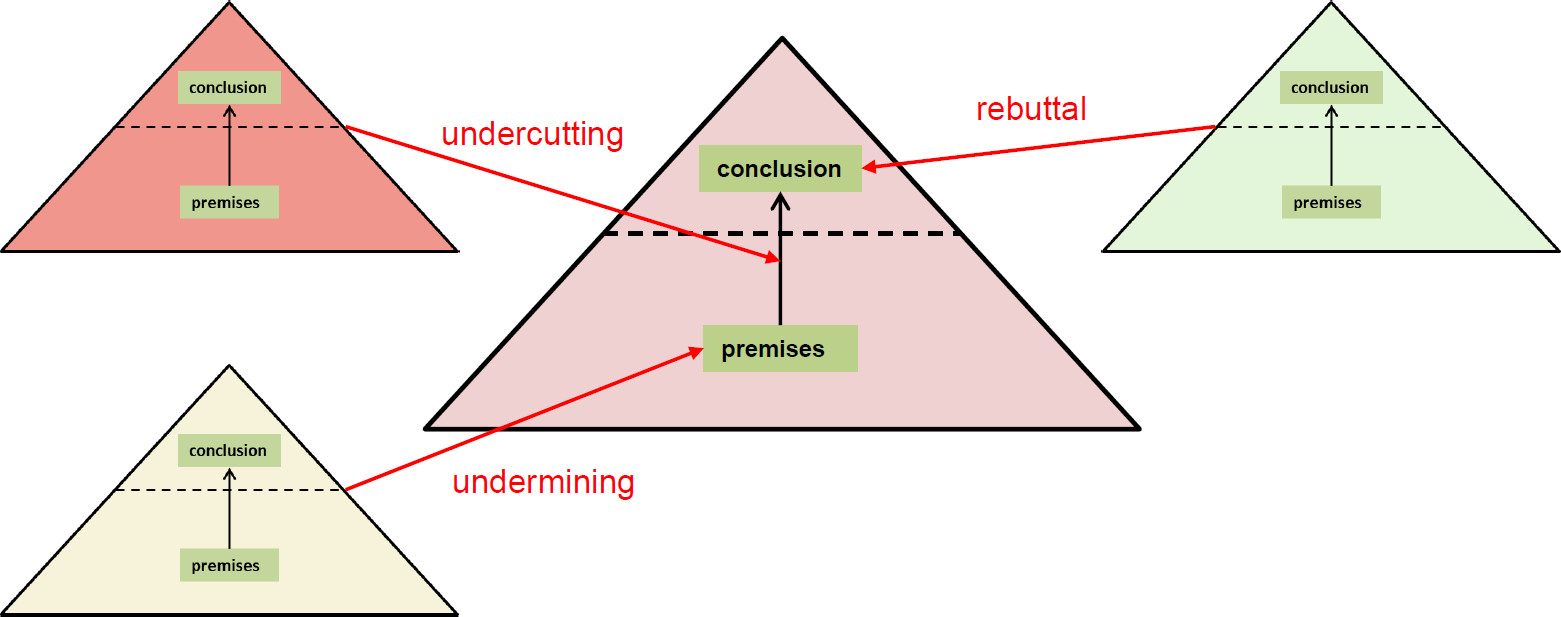
\includegraphics[width=0.8\textwidth]{Images/Argument_attacks.jpg}
    \caption{Argument attacks}
\end{figure}

While powerful, structured argumentation presents significant challenges. It is not always easy to identify all potential rebutting, undermining, and undercutting relationships. Furthermore, assessing the degree of certainty of the premises can be a complex task in itself.

\section{Abstract Argumentation}

\textbf{Abstract Argumentation} takes a different approach by abstracting away the internal content of arguments entirely. In this graph-based formalism, arguments are treated as abstract nodes, and the focus is exclusively on the attack relations between them, which are represented as directed edges in a graph. \\

The core principle of this model is to analyze the calculus of opposition. The goal is to determine what can be considered acceptable or justified based solely on the structure of the graph of conflicts. It allows researchers to reason about inconsistency and conflict at a conceptual level, regardless of the specific knowledge representation formalism used to generate the arguments. \\

Within abstract argumentation, the term "\textbf{semantics}" has a specific technical meaning: it refers to the method of evaluation used to select subsets of arguments that are collectively acceptable according to certain criteria (e.g., being conflict-free and able to defend themselves against attackers). \\

These formal models provide the symbolic and logical foundations for argumentation, but their relationship with modern, statistics-based AI is a crucial and evolving area of study.

\chapter{Argumentation and Machine Learning: A Point of Intersection}

While computational argumentation is typically a formal, symbolic branch of AI, there is a growing body of research exploring its intersection with statistical machine learning, particularly deep learning. This section addresses this relationship, highlighting the key challenges and opportunities that arise when these two distinct paradigms meet. \\

The fundamental difference between these approaches is that computational argumentation provides formal models for justification, whereas deep learning models are invariably statistical in nature. This leads to the central challenge of their integration: \textbf{Explainability}. The primary difficulty is the inherent challenge of formally justifying a conclusion drawn by a deep learning model, which often operates as a "black box." \\

Consequently, a major area of active research is not about replacing formal argumentation models with neural networks, but rather using argumentation for the explainability of machine learning models (a field known as XAI). In this framing, argumentation is positioned as a potential solution to the black box problem, offering a structured, human-comprehensible way to explain and justify the outputs of complex statistical systems. \\

In conclusion, computational argumentation is a mature field with deep roots in logic and philosophy. As AI continues to evolve, it is finding new and critical relevance in addressing the core challenges of modern systems, ensuring that as automated systems grow in power, their reasoning remains transparent, explainable, and justifiable.

\chapter{Foundational Models of Argumentation}

Computational argumentation provides a mechanism for automated reasoning where arguments can be presented, challenged, and evaluated to reach justified conclusions. This process is primarily modeled through two distinct paradigms: structured argumentation, which delves into the logical composition of arguments, and abstract argumentation, which concentrates solely on the conflict relationships between them.

\section{Structured Argumentation}

Structured argumentation examines the internal components of an argument. In this model, an argument is not an atomic entity but is composed of distinct parts, such as premises and logical rules of inference that lead to a conclusion. This approach allows for a fine-grained analysis of why an argument is valid and how it can be attacked, for instance, by challenging its premises or undermining its inference rule. A logic-based formalism is typically used to describe this internal structure, enabling a detailed, proof-based style of reasoning.

\section{Abstract Argumentation}

In contrast, abstract argumentation disregards the internal content and logical structure of arguments. This model focuses exclusively on the attack relationships that exist between arguments. The central insight is that the acceptability of an argument often depends not on its intrinsic content but on whether it can withstand attacks from other arguments. This paradigm is typically represented as a directed graph, where the nodes are arguments and the directed edges represent attacks. By analyzing the topology of this graph, one can determine which arguments emerge as justified. An example of abstract argumentation is depicted in figure 6.1.

\begin{figure}[h]
    \centering
    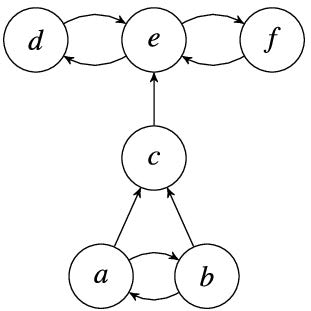
\includegraphics[width=0.3\textwidth]{Images/Abstract_argumentation.jpg}
    \caption{Abstract argumentation example}
\end{figure}

\section{Illustrative Example: Medical Reasoning}

\begin{figure}[h]
    \centering
    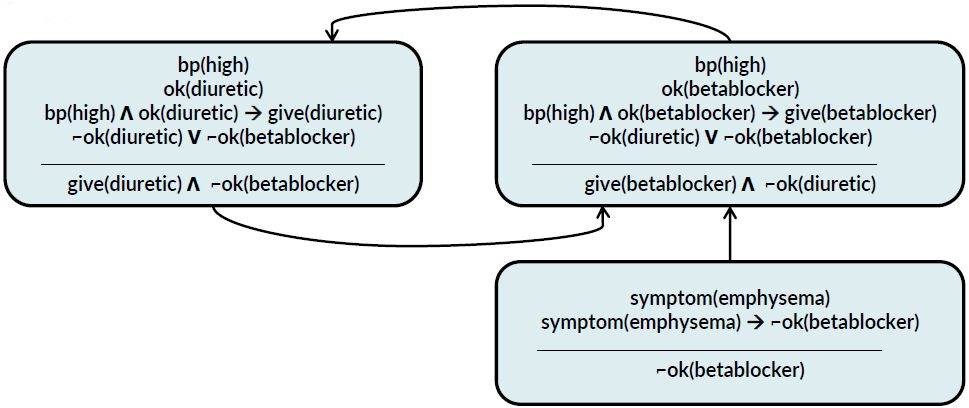
\includegraphics[width=0.5\textwidth]{Images/Structured_argumentation_example.png}
    \caption{Structured medical argumentation example}
\end{figure}

\begin{figure}[h]
    \centering
    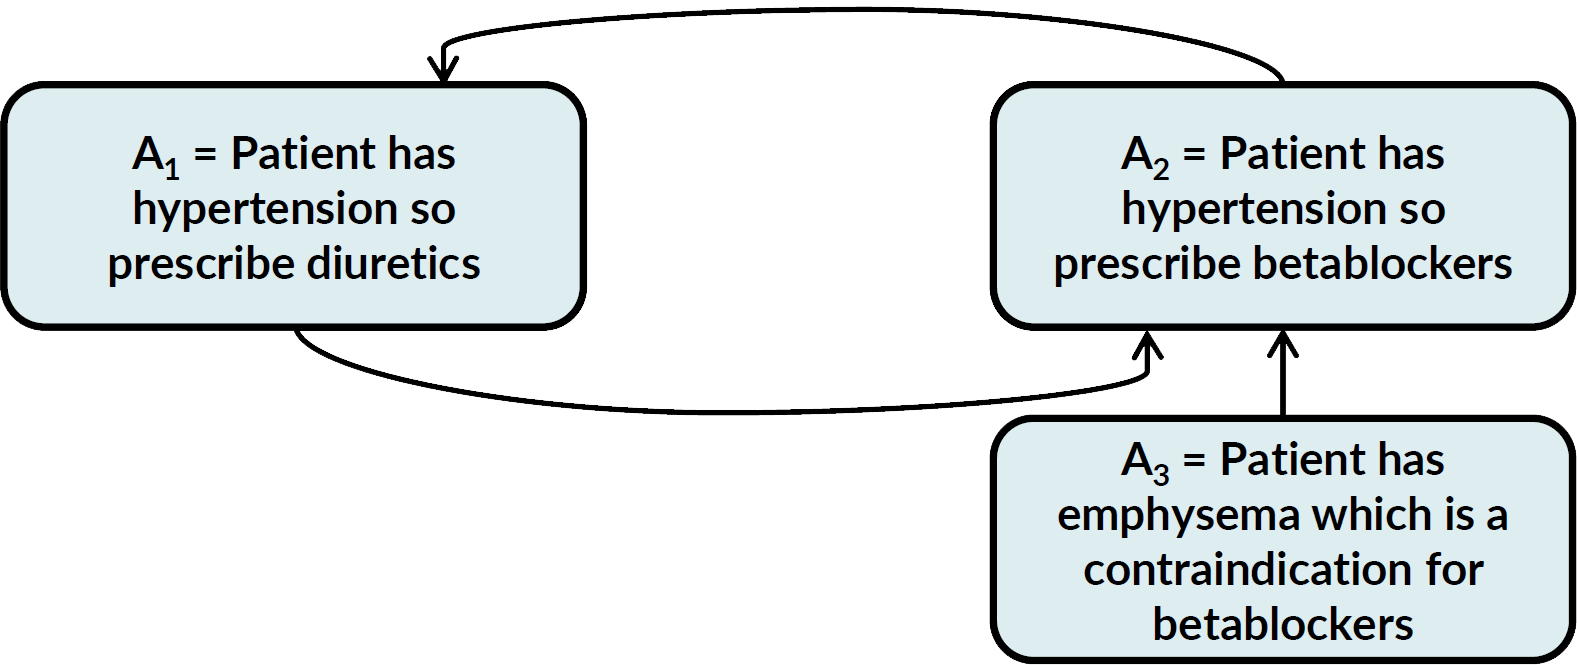
\includegraphics[width=0.5\textwidth]{Images/Abstract_argumentation_example.png}
    \caption{Abstract medical argumentation example}
\end{figure}

To differentiate these two models, consider a simplified medical reasoning scenario involving three arguments:

\begin{itemize}
    \item 
    \textbf{A1:} The patient has hypertension, so prescribe diuretics.

    \item 
    \textbf{A2:} The patient has hypertension, so prescribe beta-blockers.

    \item 
    \textbf{A3:} The patient has emphysema, which is a contraindication for beta-blockers.
\end{itemize}

A \textbf{structured approach} (figure 6.2) would analyze the logical rules and premises within each argument. For instance, it might formalize \texttt{A1} as: \texttt{$premise(hypertension) \wedge rule(hypertension \rightarrow prescribe\_diuretics) \Rightarrow conclusion(prescribe\_diuretics)$}. The conflict between \texttt{A1} and \texttt{A2} might arise from a domain constraint that only one treatment should be prescribed, while the attack from \texttt{A3} to \texttt{A2} would be based on \texttt{A3}'s conclusion directly negating a condition required for \texttt{A2} to be valid. \\

The \textbf{abstract representation} (figure 6.3), however, would ignore these internal details. It would simply model the scenario as a graph of interactions. As the source diagrams explicitly show, the arguments \texttt{A1} and \texttt{A2} attack each other, representing a mutual conflict between the two proposed treatments. Additionally, \texttt{A3} attacks \texttt{A2}, as it presents a definitive reason against the treatment proposed in \texttt{A2}. \\

\section{From SA to AA: understanding indirect attackers and supporters}

The main ideas we will expose with this example are:

\begin{enumerate}
    \item 
    What we are justified in believing is \textbf{not fixed}, but depends on the \texttt{current set of arguments and counterarguments}.

    \item 
    Each new argument can \texttt{defeat}, \texttt{reinstate}, or \texttt{re-defeat} previous conclusions.

    \item 
    Arguments can \textbf{indirectly} support or attack other arguments.
\end{enumerate}

In the figures used in this example the full lines represent support relationships while the dashed lines represent attack relationships. Green arguments are considered valid while red arguments are considered defeated. \\

Let us make an example argumentation discussing whether we should run the Large Hadron Collider and let's say that we are initially favorable to it. (See figure 6.4).

\begin{figure}[h]
    \centering
    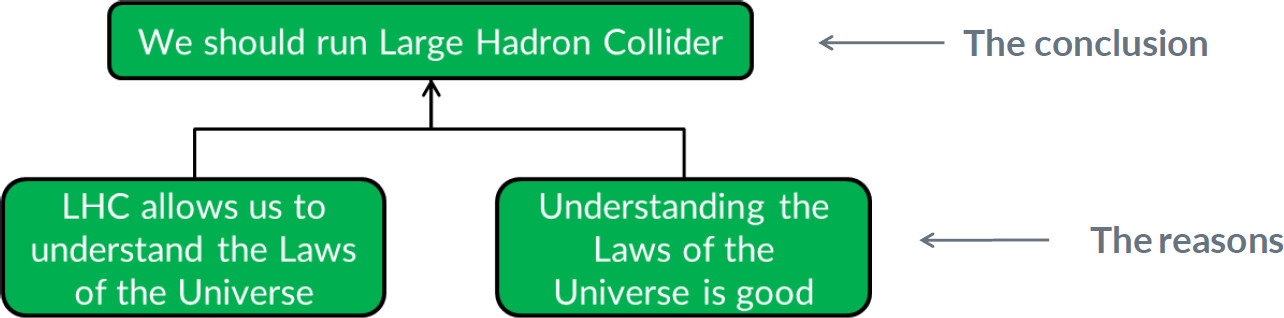
\includegraphics[width=0.5\textwidth]{Images/From_SA_to_AA_1.jpg}
    \caption{From SA to AA: Initial situation}
\end{figure}

Now, let's say that we talk about our idea to another person who disagrees with us, thus attacking our argument. At this point we are discouraged from running the LHC. (See figure 6.5).

\begin{figure}[h]
    \centering
    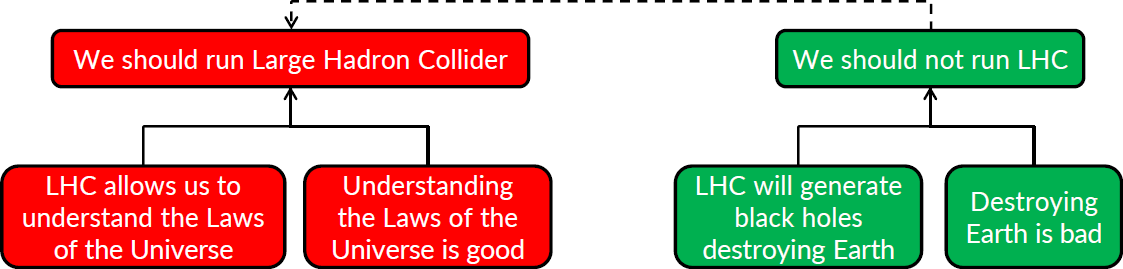
\includegraphics[width=0.5\textwidth]{Images/From_SA_to_AA_2.png}
    \caption{From SA to AA: Step 2}
\end{figure}

Now, let's say that another person overhears our conversation and joins the discussion introducing another argument that attacks one of the reasons of our attacker undermining their argument. Undermining the attacking argument reinstates our argument making it valid again. This means that the newly arrived person has indirectly supported our argument. (See figure 6.6). \\

\begin{figure}[h]
    \centering
    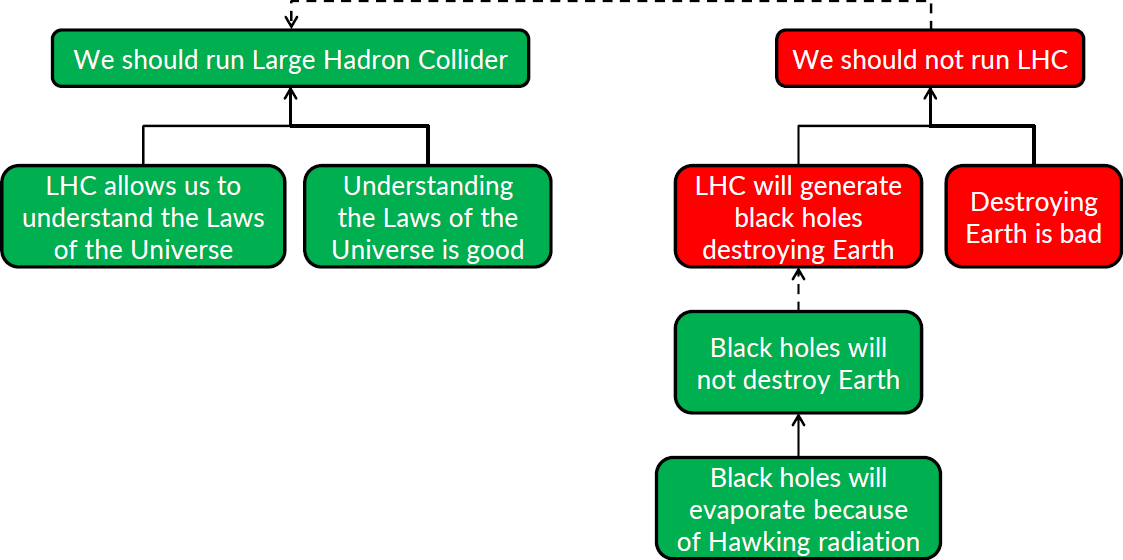
\includegraphics[width=0.5\textwidth]{Images/From_SA_to_AA_3.png}
    \caption{From SA to AA: Step 3}
\end{figure}

At this point, let's say that yet another person joins the discussion and undermines the argument that indirectly supports the initial argument. The last argument re-defeats our argument making it invalid again. (See figure 6.7). \\

\begin{figure}[h]
    \centering
    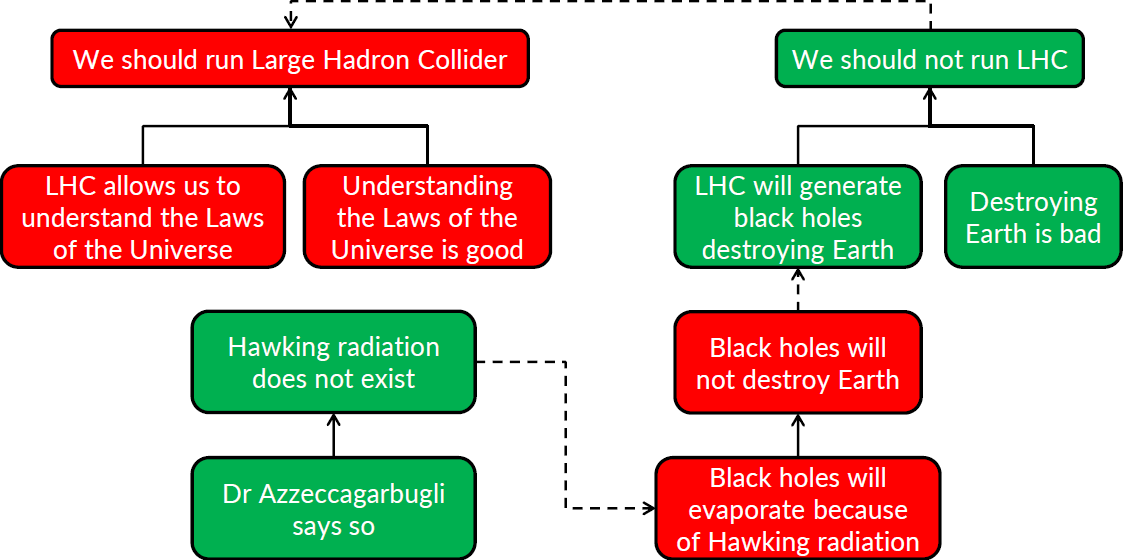
\includegraphics[width=0.5\textwidth]{Images/From_SA_to_AA_4.png}
    \caption{From SA to AA: Step 4}
\end{figure}

In the current situation, if we want to reinstate our argument we need to undermine and defeat the lastly arrived argument. Thankfully, one can attack the latter by undermining the credibility of its source. (See figure 6.8). \\

\begin{figure}[htbp]
    \centering
    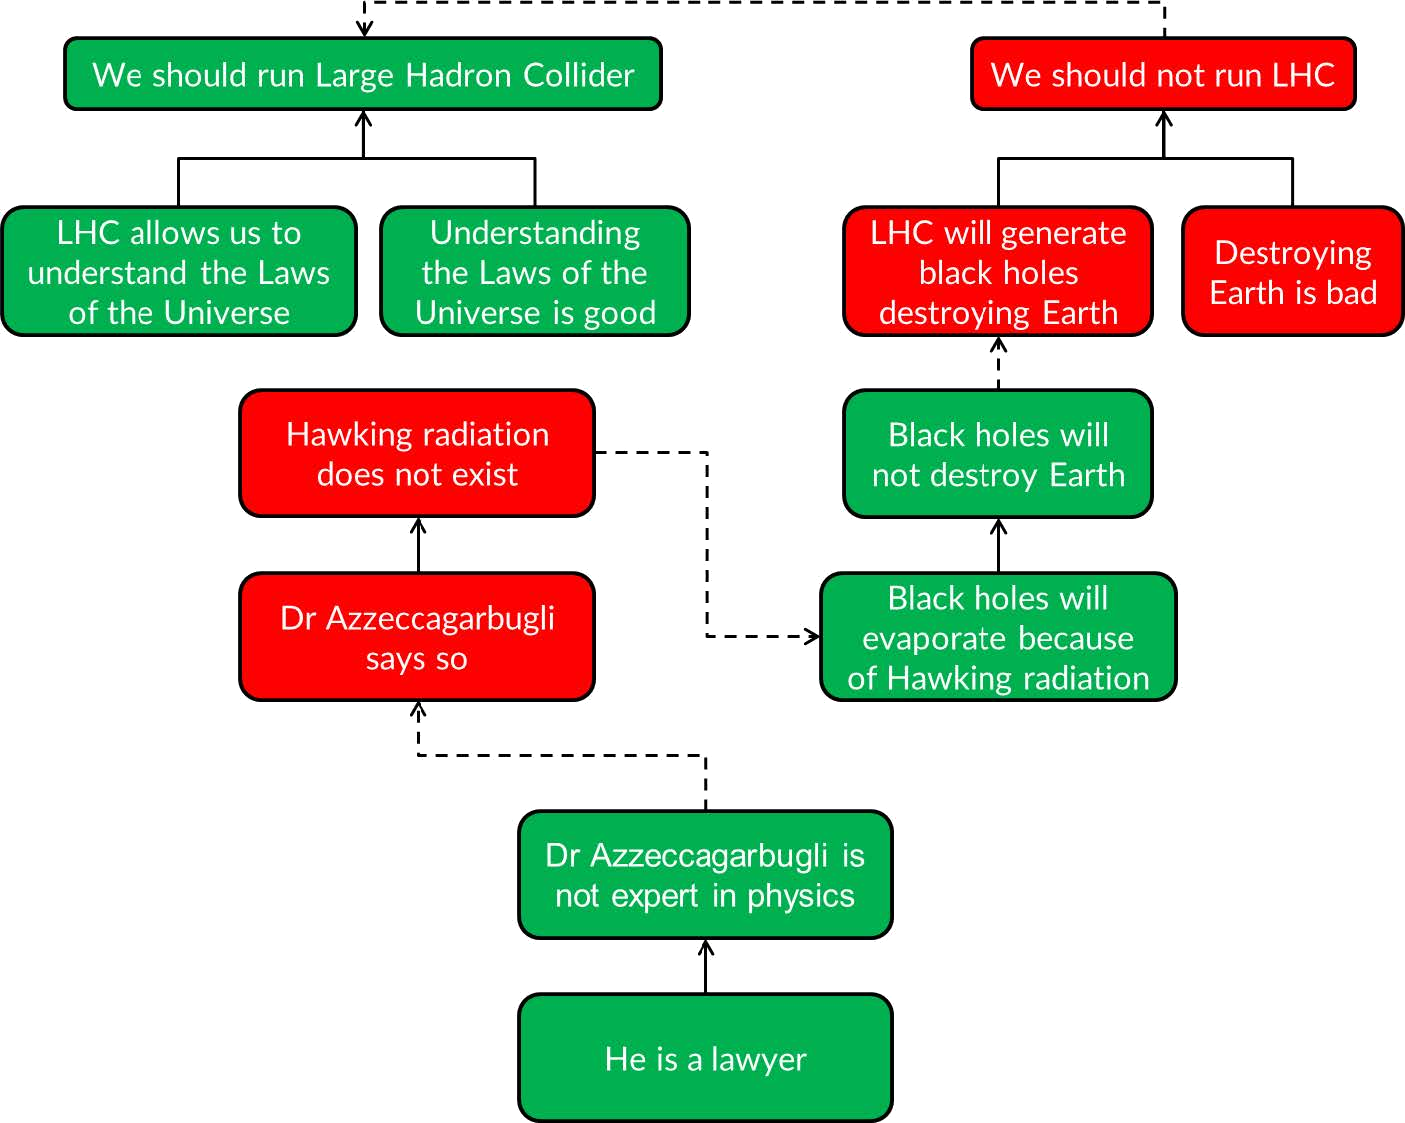
\includegraphics[width=0.5\textwidth]{Images/From_SA_to_AA_5.png}
    \caption{From SA to AA: Step 5}
\end{figure}

The examples we just exposed provide a basis for understanding structured and abstract argumentation. We will now turn to a formal definition of the most influential abstract model, which has become a cornerstone of the field.

\chapter{Dung's Abstract Argumentation Framework (AF)}

The field of abstract argumentation was revolutionized by Phan Minh Dung's seminal 1995 paper, which introduced a simple yet powerful model. This Abstract Argumentation Framework (AF) provides a formal, mathematical foundation for analyzing arguments based solely on their interactions. By abstracting away from the content of arguments, it allows for the study of conflict resolution in a general and widely applicable manner, making it a cornerstone of modern computational argumentation. In fact, the core logic of the framework can be intuitively summarized by the proverb, "He who laughs last, laughs best". An argument can attack another, but if a third argument defeats the attacker, the original argument is reinstated—it gets the "last laugh."

\section{Formal Definition}

An Argumentation Framework (AF) is formally defined as a pair consisting of a set of arguments and the attack relations between them.

An \textbf{Argumentation Framework (AF)} is a pair \texttt{$F = ⟨A, R⟩$} where:

\begin{itemize}
    \item 
    \texttt{A} is a finite set of arguments.

    \item 
    \texttt{R} is a binary "attack" relation on \texttt{A} (i.e., \texttt{$R \subseteq A \times A$}).
\end{itemize}

This formal structure is visualized as a directed graph. The arguments in the set \texttt{A} are the nodes of the graph, and the attack relations in \texttt{R} are represented as directed edges. An edge from argument \texttt{a} to argument \texttt{b} is written using the notation $aRb$ and signifies that \texttt{a} attacks \texttt{b}.

\section{The Role of Semantics}

The primary goal of analyzing an Argumentation Framework is to determine which arguments can be considered "acceptable" or justified in the context of the conflicts. This is achieved through the application of a semantics. In this context, a semantics is a set of formal criteria or rules used to identify subsets of arguments, called extensions, that can survive the conflict together. \\

Two fundamental properties underpin most semantics:

\begin{itemize}
    \item 
    \textbf{Conflict-freeness:} A set of arguments is conflict-free if no argument within the set attacks another argument in the same set. An attacking argument and its target cannot be accepted together.

    \item 
    \textbf{Defense:} An argument \texttt{a} is defended by a set of arguments \texttt{S} if, for every argument \texttt{b} that attacks \texttt{a}, there is an argument in \texttt{S} that attacks \texttt{b}. To survive, an argument must be able to counter every attack against it.
\end{itemize}

These core principles are combined in various ways to define different families of semantics, each providing a distinct perspective on what constitutes a coherent and justified set of arguments.

\chapter{Extension-Based Semantics}

\begin{figure}[h]
    \centering
    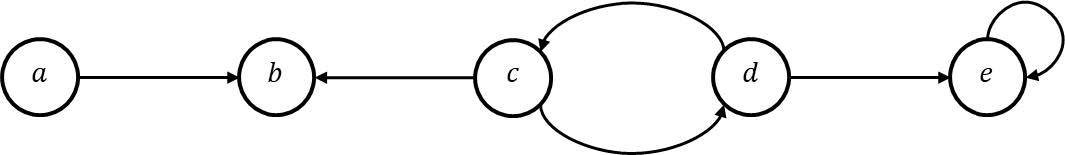
\includegraphics[width=0.8\textwidth]{Images/Abstract_argumentation_graph.jpg}
    \caption{Reference graph to expose the extension-based semantics}
\end{figure}

The most established family of methods for evaluating argumentation frameworks is known as extension-based semantics. The core principle of this approach is to evaluate arguments on a binary basis: each argument is either accepted or rejected. The goal is to identify one or more coherent sets of winning arguments, known as extensions. In this paradigm, a single undefended attack is sufficient to "kill" or defeat an argument, removing it from consideration. \\

The following definitions outline the key extension-based semantics, each built upon specific combinations of properties like conflict-freeness and defense. \\

We will expose the semantics using figure 8.1 as a reference graph.

\section{Conflict-Free Sets}

A set is conflict-free if it contains \textbf{no internal conflicts}. This is the most basic property required for a set of arguments to be considered jointly acceptable. \\

Formally, we say that: $S$ is conflict free if $\nexists$ $a, b \in S$ s.t. $aRb$. \\

The conflict free sets of the reference graph are the following: \\

$cf(F) = \{\{a,c\}, \{a,d\}, \{b,d\},\{a\},\{b\},\{c\},\{d\},\emptyset \}$ \\

Let us explain the conflict-free sets gradually in ascending order of number of elements:

\begin{itemize}
    \item
    The $\emptyset$ is conflict-free by definition because, in order for a conflict to exist, there must be an attack between arguments which imply the presence of at least a self attacking argument. If there aren't arguments in the set, there cannot be a conflict.

    \item 
    Sets which contain a single element are conflict-free if the single element does not attack itself. Arguments $a, b, c$ and $d$ are not self attacking while argument $e$ is.

    \item 
    Sets which contain more than one element are conflict-free if none of the elements of a set attacks another element of the same set. For instance, the set $\{a,c\}$ fulfills this requirement. Other sets like $\{a,b\}$ and $\{c,d\}$ do not fulfill this requirement because $a$ attacks $b$ and $c$ and $d$ attack each other. In the considered example we can't have a set containing 3 arguments because $b$ is attacked both by $a$ and $c$ and $c$ and $d$ attack each other.
\end{itemize}

\section{Admissible Sets}

An admissible set is a conflict-free set that also \textbf{defends all of its arguments} against external attacks. This captures the intuition that a justified viewpoint must be internally consistent and capable of countering all challenges. \\

Formally, we say that: $S$ is admissible if $S$ is conflict-free and $S$ is defended by itself, i.e. $\forall a \in S, \forall b \in A, bRa \Rightarrow \exists$ $c \in S$ s.t. $cRb$. \\

According to the definition of admissible sets, we can create the set of admissible sets by starting from the conflict-free sets and removing its non-compliant elements. Before we expose the skimming process in table 8.1 we need to introduce the definition of \textbf{vacuous protection}. \\

We say that an element is \textbf{vacuously protected} if it doesn't have attacking arguments. \\

The admissible sets of the considered example are: \\

$adm(F) = \{\{a,c\},\{a,d\},\{a\},\{c\},\{d\},\emptyset\}$ \\

\begin{table}
    \begin{tabularx}{\linewidth}{|p{5em}|p{4em}|X|} \hline
         \textbf{Element} & \textbf{Kept?} & \textbf{Reason} \\ \hline

        $\emptyset$ & Yes &
        We keep the empty set because it has no elements and none can attack it. Hence, it counts as vacuously protected. \\ \hline

        $\{a\}$ & Yes &
        $\{a\}$ is vacuously protected because it does not have attacking arguments. \\ \hline

        $\{b\}$ & No &
        $b$ is attacked by $a$ and $c$ but the set $\{b\}$ does not contain elements that attack $a$ and $c$. This means that the set $\{b\}$ is not defended by itself.\\ \hline

        $\{c\}$ & Yes &
        $c$ is attacked by $d$ and the set $\{c\}$ contains an element ($c$) that attacks the attacker $d$. Hence, the set $\{c\}$ is defended by itself.\\ \hline

        $\{d\}$ & Yes &
        Similarly to $\{c\}$, the set contains an element that attacks its attacker. \\ \hline

        $\{a,c\}$ & Yes &
        The set contains the element $c$ which is attacked by $d$ but, at the same time, $c$ attacks its attacker $d$ defending itself. \\ \hline

        $\{a,d\}$ & Yes &
        This case is analogous to $\{a,c\}$.\\ \hline

        $\{b,d\}$ & No &
        $b$ is attacked by $a$ and $c$ and $d$ is attacked by $c$. This means that this set has 2 attackers: $a$ and $c$. $d$ attacks $c$ defending itself and $b$ but nobody attacks $a$ and this leaves $b$ exposed to the attacks of $a$. This means that this set does not fully defend itself.\\ \hline
    \end{tabularx}
    \caption{Admissible sets explanation}
\end{table}

\section{Naive Extensions}

A naive extension represents a \textbf{maximal conflict-free set}. This means it is a conflict-free set to which no other argument from the framework can be added without introducing a conflict. The name "naive" derives from the fact that it captures a very intuitive notion of acceptability; one might be satisfied with this simple idea of a maximally consistent viewpoint without considering defense. \\

Formally, we say that: $S$ is a naive extension if $S$ is conflict-free and $\nexists T \in cf(F)$ s.t. $T\supset S$. \\

According to the formal mathematical definition of naive extension we can start from the conflict-free set and select only its elements which do not have a proper superset. The skimming process is exposed in table 8.2.\\

$naive(F) = \{\{a,c\},\{a,d\},\{b,d\}\}$

\begin{table}[]
    \begin{tabularx}{\linewidth}{|p{5em}|p{4em}|X|} \hline
         \textbf{Element} & \textbf{Kept?} & \textbf{Reason} \\ \hline

        $\emptyset$ & No &
        The empty set is a subset of all sets and hence, all the other sets in the conflict-free sets are proper supersets of its. \\ \hline

        $\{a\}$ & No &
        $\{a,c\}$ and $\{a,d\}$ are proper supersets of $\{a\}$.\\ \hline

        $\{b\}$ & No &
        $\{b,d\}$ is a proper superset of $\{b\}$.\\ \hline

        $\{c\}$ & No &
        $\{a,c\}$ is a proper superset of $\{c\}$.\\ \hline

        $\{d\}$ & No &
        $\{b,d\}$ is a proper superset of $\{d\}$.\\ \hline

        $\{a,c\}$ & Yes &
        $\{a,c\}$ does not have a proper superset in  $cf(F)$.\\ \hline

        $\{a,d\}$ & Yes &
        This case is analogous to $\{a,c\}$.\\ \hline

        $\{b,d\}$ & Yes &
        This case is analogous to $\{a,c\}$.\\ \hline
    \end{tabularx}
    \caption{Naive extension explanation}
\end{table}

\section{Complete Extensions}

A complete extension is an admissible set that also contains \textbf{all the arguments it defends}. This property, known as reinstatement, ensures that if a set of arguments successfully defends an external argument, that argument is brought "on board" and included in the extension. This means that we can create the complete extensions starting from the admissible sets and discarding the non-compliant sets. The skimming process is exposed in table 8.3.\\

$comp(F) = \{\{a,c\},\{a,d\},\{a\}\}$ \\

\begin{table}
    \begin{tabularx}{\linewidth}{|p{5em}|p{4em}|X|} \hline
         \textbf{Element} & \textbf{Kept?} & \textbf{Reason} \\ \hline

        $\emptyset$ & No &
        \textit{The empty set is not considered a complete extension if the graph contains unattacked arguments.}
        The graph contains the unattacked element $a$. An unattacked element is considered to be protected by all sets including $\emptyset$. According to the reinstatement property, $\emptyset$ would be a complete extension if it contained $a$. But it doesn't.\\ \hline

        $\{a\}$ & Yes &
        $a$ attacks $b$ but $b$ doesn't attack another argument. Formally, we can say that $a$ defends $\emptyset$ which is already included in $\{a\}$.\\ \hline

        $\{c\}$ & No &
        $c$ attacks $d$ which in turn attacks $e$. This means that $c$ defends $e$. In order for the set $\{c\}$ to be a complete extension it should also contain $e$ but it doesn't.\\ \hline

        $\{d\}$ & No &
        $d$ attacks $c$ and $e$. $e$, in turn, attacks itself and, considering that the attacker of the attacker is a protector, $d$ protects $e$.
        As for $c$, it attacks $b$ and this means that $d$ protects $b$. According to the reinstatement principle $\{d\}$ would have to include $c$ and $e$ but it doesn't.\\ \hline

        $\{a,c\}$ & Yes &
        The set $\{a,c\}$ is attacked by argument $d$ which is, in turn, attacked by $c$ which is part of the set $\{a,c\}$. This means that the set contains all the arguments it defends.\\ \hline

        $\{a,d\}$ & Yes &
        The set $\{a,d\}$ is attacked by argument $c$ which is, in turn, attacked by $d$ which is part of the set $\{a,d\}$. This means that the set contains all the arguments it defends.\\ \hline
    \end{tabularx}
    \caption{Complete extensions explanation}
\end{table}

\section{Grounded Extensions}

The grounded extension is the \textbf{minimal complete extension}. It represents the most skeptical or cautious viewpoint, containing only those arguments that are universally agreed upon and incontrovertibly justified. It can be seen as a kernel of arguments from which nothing can be removed without violating completeness. Formally, we say that the grounded extensions verify the \textbf{strong admissibility} property. i.e. a grounded extension does not contain self-defeating arguments. \\

According to the formal definition of the grounded extensions, we can derive them starting from the complete extensions and discarding the non compliant elements. The skimming process is exposed in table 8.4.\\

$grd(F) = \{\{a\}\}$

\begin{table}
    \begin{tabularx}{\linewidth}{|p{5em}|p{4em}|X|} \hline
         \textbf{Element} & \textbf{Kept?} & \textbf{Reason} \\ \hline

        $\{a\}$ & Yes &
        $\{a\}$ is a minimal complete extension because it has 2 supersets in $comp(F)$\\ \hline

        $\{a,c\}$ & No &
        $\{a,c\}$ is a superset of $\{a\}$\\ \hline

        $\{a,d\}$ & No &
        $\{a,d\}$ is a superset of $\{a\}$\\ \hline
    \end{tabularx}
    \caption{Grounded extensions explanation}
\end{table}

\section{Preferred Extensions}

A preferred extension is a \textbf{maximal admissible set}. It represents a credulous but still consistent viewpoint. A framework can have multiple preferred extensions, representing different, equally valid perspectives on the conflict. Each one is a coherent position that cannot be expanded further without becoming vulnerable to attacks. \\

Formally, we say that: $S$ is a preferred extension if $S$ is admissible and $\nexists T \in adm(F) s.t. T \supset S$. \\

Informally, we say that the preferred extensions are the sets in $adm(F)$ which do not have a proper superset. This means that we can derive $pref(F)$ starting from $adm(F)$ and removing the non-compliant elements. The skimming process is exposed in table 8.5.\\

$pref(F) = \{\{a,c\},\{a,d\}\}$

\begin{table}
    \begin{tabularx}{\linewidth}{|p{5em}|p{4em}|X|} \hline
         \textbf{Element} & \textbf{Kept?} & \textbf{Reason} \\ \hline

        $\emptyset$ & No &
        All the sets are supersets of $\emptyset$.\\ \hline

        $\{a\}$ & No &
        $\{a,c\}$ and $\{a,d\}$ are supersets of $\{a\}$.\\ \hline

        $\{c\}$ & No &
        $\{a,c\}$ is a superset of $\{c\}$.\\ \hline

        $\{d\}$ & No &
        $\{a,d\}$ is a superset of $\{d\}$.\\ \hline

        $\{a,c\}$ & Yes &
        $\{a,c\}$ does not have a proper superset in $adm(F)$.\\ \hline

        $\{a,d\}$ & Yes &
        $\{a,d\}$ does not have a proper superset in $adm(F)$.\\ \hline
    \end{tabularx}
    \caption{Preferred extensions explanation}
\end{table}

\section{Stable Extensions}

A stable extension is a conflict-free set that \textbf{attacks every argument not included in the set}. This represents a highly dominant and stable viewpoint that not only defends itself but also actively invalidates every competing argument in the framework. This makes it a particularly strong form of acceptability, but it is also a difficult property to achieve, and many frameworks do not have a stable extension. \\

Formally, we say that: $S$ is a stable extension if $S$ is conflict-free and $\forall a \in A \smallsetminus S$ $\exists b \in S$ s.t. $bRa$. \\

Informally, we say that the stable extensions are all the conflict-free sets which attack all the elements not belonging to the set. This means that we can derive the stable extensions starting from the conflict free sets and discarding all the elements which do not attack all the external elements. The skimming process is exposed in table 8.6.\\

$stb(F) = \{\{a,d\}\}$ \\

\begin{table}[]
    \begin{tabularx}{\linewidth}{|p{5em}|p{4em}|X|} \hline
         \textbf{Element} & \textbf{Kept?} & \textbf{Reason} \\ \hline

        $\emptyset$ & No &
        The empty set does not have elements and, therefore, it cannot attack other arguments.\\ \hline

        $\{a\}$ & No &
        The set $\{a\}$ attacks only $b$. It does not attack all the other arguments.\\ \hline

        $\{b\}$ & No &
        The set $\{b\}$ does not attack anyone.\\ \hline

        $\{c\}$ & No &
        The set $\{c\}$ attacks only $b$ and $d$. It does not attack the other arguments.\\ \hline

        $\{d\}$ & No &
        The set $\{d\}$ attacks only $c$ and $e$. It does not attack the other arguments.\\ \hline

        $\{a,c\}$ & No &
        The set $\{a,c\}$ attacks the arguments $b$ and $d$ but it leaves the argument $e$ unattacked.\\ \hline

        $\{a,d\}$ & Yes &
        The set $\{a,d\}$ attacks all the other arguments in the framework which are external to the set.\\ \hline

        $\{b,d\}$ & No &
        The set $\{b,d\}$ attacks the arguments $c$ and $e$ but it leaves the argument $a$ unattacked.\\ \hline
    \end{tabularx}
    \caption{Stable extensions explanation}
\end{table}

The binary nature of these semantics, while powerful, can be limiting in scenarios requiring a more nuanced assessment. This has led to the development of an alternative approach that offers a more granular evaluation of argument strength.

\chapter{Ranking-Based Semantics}

\begin{figure}[h]
    \centering
    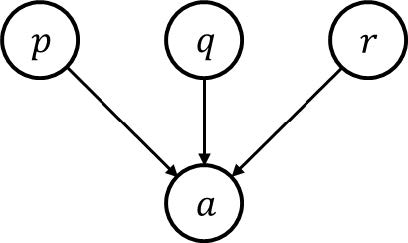
\includegraphics[width=0.4\textwidth]{Images/Ranking_based_semantics_graph.jpg}
    \caption{Example of real-world debate}
\end{figure}

Ranking-based semantics were developed to address the limitations of the binary accept/reject model. Instead of making a categorical decision, this approach provides a gradual, often numerical, level of acceptability for each argument. The final output is a ranking that orders the arguments from most to least acceptable. This is particularly useful in scenarios where multiple attacks should have a cumulative weakening effect. For example, consider an argument \texttt{a}: "She is the best candidate for the position," which is attacked by three separate counterarguments: \texttt{p} ("She lacks teaching experience"), \texttt{q} ("She has no publications in the area"), and \texttt{r} ("She does not speak English"). In an extension-based model, one of these attacks, if undefended, would be enough to "kill" argument \texttt{a}. A ranking-based approach, however, intuits that three attacks should weaken \texttt{a} more than just one, providing a more realistic depiction of many real-world debates. \\

The fundamental differences between the two semantic paradigms is summarized in table 9.1.

\begin{table}
    \centering
    \begin{tabularx}{\textwidth}{|X|X|X|} \hline
        \textbf{Principle} & \textbf{Extension-based Semantics} & \textbf{Ranking-based Semantics} \\ \hline

        Acceptability Status & Arguments are either accepted or rejected (binary). & 
        Provides gradual levels of acceptability (e.g., a numerical score). \\ \hline

        Effect of Attacks & Defeated arguments are "killed" and excluded. & 
        Attacked arguments are "weakened" but not eliminated. \\ \hline

        Relevance of Attack Count & The number of undefended attacks is irrelevant; one is enough. & 
        The more attacks an argument receives, the lower its acceptability. \\ \hline

        Nature of Status & Status is absolute (accepted or rejected). & 
        Degrees of acceptability are relative and used for comparison. \\ \hline

        Comparability of Accepted Arguments & All accepted arguments share the same level of acceptability. & 
        Enables a full ranking of arguments from most to least acceptable. \\ \hline
    \end{tabularx}
    \caption{Semantic paradigms comparison}
\end{table}

\section{Foundational Properties}

Ranking-based semantics are often characterized by a set of desirable properties that guide their design and behavior. Key properties include:

\begin{itemize}
    \item 
    \textbf{Abstraction (Abs):} The ranking of arguments is determined solely based on the attack graph, without considering the internal content of the arguments.

    \item 
    \textbf{Independence (In):}  The ranking between two arguments \texttt{a} and \texttt{b} should be independent of any argument that is neither connected to \texttt{a} nor to \texttt{b}.

    \item 
    \textbf{Void Precedence (VP):} Any non-attacked argument must be ranked strictly higher than any argument that is attacked.

    \item 
    \textbf{Self-Contradiction (SC):} A self-attacking argument must be ranked lower than any argument that is not self-attacking.

    \item 
    \textbf{Cardinality Precedence (CP):} The acceptability of an argument decreases as the number of arguments directly attacking it increases.
\end{itemize}

\chapter{Key Algorithms and Semantics}

\begin{figure}[h]
    \centering
    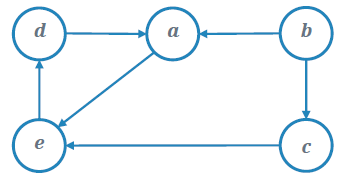
\includegraphics[width=0.4\textwidth]{Images/Ranking-based_reference_graph.png}
    \caption{Reference graph to expose the ranking-based algorithms}
\end{figure}

Several algorithms have been proposed to implement ranking-based semantics and we will expose them using the graph in figure 10.1. The algorithms exposed in the following sections are among the most notable. \\

Before we proceed with the expositions we have to clarify the notation used henceforth. We classify the attack relations to a node \texttt{a} according to their contribution to its acceptability. If an attack relation contributes negatively to the acceptability of node \texttt{a} we put it in the set of the negative attack relations identified with $R^-(a)$. If it contributes positively, instead, we put it in the set of the positive attack relations identified with $R^+(a)$. The subscript number of the attack relations $R$ is used to indicate either the number of nodes or the number of edges  involved in the attack path towards the target argument.

\section{Categorizer}

The Categorizer semantic assigns a numerical score, typically between 0 and 1, to each argument. The score of an argument is inversely related to the sum of the scores of its attackers. Unattacked arguments receive a maximal score of 1. The scores for all other arguments are typically found by defining and solving a system of equations. \\

The score for an argument \texttt{a} is defined as:
\[
    Cat(a) =
    \begin{cases}
        1 & \text{if a is unattacked}\\
        \dfrac{1}{1 + \sum_{b\in R^-_1(a)}Cat(b)} & \text{otherwise} \\
    \end{cases}
\] \\

In the case of the categorizer, the subscript number of the attack relation indicates the number of edges involved in the attack path. So, $ R^-_1(a)$ is the set of direct attackers of the argument $a$. \\

Let us calculate the categorizer scores for all the nodes in the graph:

\begin{enumerate}[label=\alph*)]
    \item
    The argument \texttt{a} has two direct attackers: \texttt{b} and \texttt{d}. This means that $Cat(a) = \frac{1}{1 + Cat(b) + Cat(d)}$.

    \item 
    The argument \texttt{b} doesn't have attackers, so $Cat(b) = 1$.

    \item 
    The argument \texttt{c} is only attacked by \texttt{b}. So, $Cat(c) = \frac{1}{1 + Cat(b)}$.

    \item 
    The argument \texttt{d} is only attacked by \texttt{e}. So, $Cat(d) = \frac{1}{1 + Cat(e)}$.

    \item 
    The argument \texttt{e} has two direct attackers: \texttt{a} and \texttt{c}. This means that $Cat(e) = \frac{1}{1 + Cat(a) + Cat(c)}$.
\end{enumerate}

We can find the categorizer value of the arguments by solving a system of equations:

\[
    \begin{aligned}
        \begin{cases}
            Cat(a) = \frac{1}{1 + Cat(b) + Cat(d)} \\
            Cat(b) = 1 \\
            Cat(c) = \frac{1}{1 + Cat(b)} \\
            Cat(d) = \frac{1}{1 + Cat(e)} \\
            Cat(e) = \frac{1}{1 + Cat(a) + Cat(c)}
        \end{cases}
        \;&\Rightarrow\;
        \begin{cases}
            Cat(a) \approx 0.38 \\
            Cat(b) = 1 \\
            Cat(c) = 0.5 \\
            Cat(d) \approx 0.65 \\
            Cat(e) \approx 0.53
        \end{cases}
    \end{aligned}
\] \\

After finding the categorizer values, we can use them to sort the arguments in descending order. \\

$b >^{Cat} d >^{Cat} e >^{Cat} c >^{Cat} a$

\section{Discussion-based Semantics (Dbs)}

This method ranks arguments by analyzing attack paths, or "discussions", ending in the node under consideration. Attack paths are classified according to the number \texttt{i} of nodes involved and we generate attack paths until all arguments have a different array of discussion values so that we can sort them using a unique lexicographical order. \\

The discussion value for an argument \texttt{a} at path length \texttt{i} is:

\[
    Dis_i(a) = 
    \begin{cases}
        -\|R_i^+(a)\| & \text{if i is odd} \\
        \|R_i^-(a)\| & \text{if i is even} \\
    \end{cases}
\] \\

Let us analyze the cases in which \texttt{i} is odd and explain why they are favorable. If $i=1$ we only have the considered argument in the path and arguments are inherently self-supporting. If $i=3$ we have the following situation: $A_3 \rightarrow A_2 \rightarrow A_1$. We have that $A_2$ attacks $A_1$ and $A_3$ attacks $A_2$ supporting $A_1$ indirectly. The same reasoning can be applied to all paths involving an odd number of nodes ending in the node under consideration. \\

Paths involving an even number of nodes, instead, are unfavorable because they undermine the validity of an argument. For example, if $i=2$ we have that $A_2 \rightarrow A_1$ and if $i=4$ we have that $A_4 \rightarrow A_3 \rightarrow A_2 \rightarrow A_1$. In the latter case we have that $A_4$ attacks $A_3$ which is an indirect supporter of $A_1$ and thus $A_4$ attacks $A_1$. The same reasoning can be applied to all paths of even length. \\

If there are self-attacking arguments they count both as attackers and supporters of themselves because we have to consider the paths ending in the given node. \\

Now, let us compute the discussion score of all the arguments in the reference graph.

\begin{enumerate}
    \item 
    For $i=1$ we have that all the paths ending in a given node only involve the given node itself. So, $-\|R_1^+(n)\| = -1$ $\forall n \in A$ and the discussion arrays are $Dis(n) = [-1]$ $\forall n \in A$. Considering that all the nodes have the same discussion array, we can't create a unique lexicographical order and we have to increase the value of \texttt{i} to add elements to them.

    \item 
    For $i=2$ we have to consider the paths involving two nodes which end in the argument under consideration. Basically we have to count the direct attackers of the given argument.
    \begin{enumerate}[label=\alph*)]
        \item 
        Argument \texttt{a} has two direct attackers: \texttt{b} and \texttt{d}. So, $\|R_2^-(a)\|=2$ and $Dis(a)=[-1,2]$.

        \item 
        Argument \texttt{b} does not have direct attackers. So, $\|R_2^-(b)\|=0$ and $Dis(b)=[-1,0]$.

        \item 
        Argument \texttt{c} is attacked only by \texttt{b}. So, $\|R_2^-(c)\|=1$ and $Dis(c)=[-1,1]$.

        \item 
        Argument \texttt{d} is attacked only by argument \texttt{e}. So, $\|R_2^-(d)\|=1$ and $Dis(d)=[-1,1]$.

        \item 
        Argument \texttt{e} is attacked by arguments \texttt{a} and \texttt{c}. So $\|R_2^-(e)\|=2$ and $Dis(a)=[-1,2]$.
    \end{enumerate}

    At this point we still can't create a unique lexicographical order for the arguments because $Dis(a)=Dis(e)$ and $Dis(c)=Dis(d)$.

    \item 
    For $i=3$ we have to count the paths involving 3 nodes that end in the argument under consideration. We can identify these paths by inspection: we start from the argument under consideration and check if there are incoming arcs. If there are incoming arcs, we move to the origin of the arcs and repeat the process. For instance, argument \texttt{a} has 2 incoming arcs originating in \texttt{b} and \texttt{d}. Let us start from the arc originating in \texttt{b}. We move to \texttt{b} and check if there are incoming arcs. There aren't, so it's impossible to form a path of 3 nodes passing from \texttt{b}. Now, let us move to argument \texttt{d} and check if there are incoming arcs. The only incoming arc originates in node \texttt{e} so, it is possible to form a 3-nodes path ending in \texttt{a}.
    \begin{enumerate}[label=\alph*)]
        \item 
        Argument \texttt{a} only has one 3-nodes incoming path. So, $-\|R_3^+(a)\| = -1$ and $Dis(a)=[-1,2,-1]$.

        \item 
        Argument \texttt{b} does not have attackers. So, $-\|R_3^+(b)\| = 0$ and $Dis(b)=[-1,0,0]$.

        \item 
        Argument \texttt{c} does not have 3-nodes attacking paths. So, $-\|R_3^+(c)\| = 0$ and $Dis(c)=[-1,1,0]$.

        \item 
        Argument \texttt{d} has 2 3-nodes attacking paths ($a \rightarrow e \rightarrow d$ and $c \rightarrow e \rightarrow d$). So, $-\|R_3^+(d)\| = -2$ and $Dis(d)=[-1,1,-2]$.

        \item 
        Argument \texttt{e} has 3 3-nodes attacking paths ($b \rightarrow a \rightarrow e$, $d \rightarrow a \rightarrow e$ and $b \rightarrow c \rightarrow e$). So, $-\|R_3^+(e)\| = -3$ and $Dis(e)=[-1,2,-3]$.
    \end{enumerate}

    For $i=3$ we have that all the discussion arrays are different, so we can create a unique lexicographical order. The discussion arrays are reported in table 10.1.
\end{enumerate}

\begin{table}[]
    \centering
    \begin{tabular}{|r|c|c|c|} \hline
         &  $i=1$ & $i=2$ & $i=3$ \\ \hline

        $Dis(a)=$ & $-1$ & $2$ & $-1$ \\ \hline
        $Dis(b)=$ & $-1$ & $0$ & $0$ \\ \hline
        $Dis(c)=$ & $-1$ & $1$ & $0$ \\ \hline
        $Dis(d)=$ & $-1$ & $1$ & $-2$ \\ \hline
        $Dis(e)=$ & $-1$ & $2$ & $-3$ \\ \hline
    \end{tabular}
    \caption{Discussion arrays}
\end{table}

To sort the arrays in lexicographical order we have to imagine that we are sorting words in alphabetical order but instead of having words we have arrays and instead of having letters we have numbers. \\

The first element of the discussion array is the same for everyone, so we can move on to the second element. The second element of the arrays can have values $0$, $1$ or $2$. So, for now, we can sort the discussion arrays in ascending order of their second element.

\begin{enumerate}
    \item 
    $b: Dis(b)=[-1,0]$

    \item 
    $c: Dis(c)=[-1,1]$

    \item 
    $d: Dis(d)=[-1,1]$

    \item 
    $a: Dis(a)=[-1,2]$

    \item 
    $e: Dis(e)=[-1,2]$
\end{enumerate}

This lexicographical order is not unique because we could swap \texttt{c} with \texttt{d} and \texttt{a} with \texttt{e} and still have the same order. To break the tie between \texttt{c} and \texttt{d} and between \texttt{a} with \texttt{e} we introduce the third elements of the discussion arrays. \\

The possible values of the third elements are $-3$, $-2$, $-1$ and $0$. It's true that there are two instances of the value $0$ but one belongs to the array of \texttt{b} which does not have a tie with another argument. So, now we can finally create a unique lexicographical order as follows:

\begin{enumerate}
    \item 
    $b: Dis(b)=[-1,0,0]$

    \item 
    $d: Dis(d)=[-1,1,-2]$

    \item 
    $c: Dis(c)=[-1,1,0]$

    \item 
    $e: Dis(e)=[-1,2,-3]$

    \item 
    $a: Dis(a)=[-1,2,-1]$
\end{enumerate}

In conclusion, we can say that according to the Discussion-based Semantics: \\

$b >^{Dbs} d >^{Dbs} c >^{Dbs} e >^{Dbs} a$

\section{Burden-based Semantics (Bbs)}

This method assigns a "burden number" to each argument, representing the difficulty of its acceptance. The calculation is iterative (indexed by step \texttt{i}): at each step, an argument's burden is based on the burden numbers of its attackers from the previous step. The key insight is that an attacker with a high burden number is "not an effective attacker", which is captured by using the reciprocal of its burden number in the calculation. A lower burden number signifies higher acceptability. \\

The burden number for an argument \texttt{a} at step \texttt{i} is:

\[
    Bur_i(a) =
    \begin{cases}
        1 & \text{if $i = 0$} \\
        1 + \sum_{b \in R_1^-(a)}\frac{1}{Bur_{i-1}(b)} &
        \text{otherwise}
    \end{cases}
\] \\

In the Burden-based Semantics the subscript number of $Bur$ indicates the iteration of the algorithm. We start generating values from $i=1$ and, in order to generate the value of the current iteration, we have to refer to the burden values of the previous one.
This means that we need a burden value for the arguments at step $0$, so we assign a default value of $1$.
As for the subscript value of $R^-$, it indicates the length of the path ending in the node under consideration. In this algorithm we have a fixed subscript of $1$ indicating that we have to consider the direct attackers of the given node at each step. \\

As we did in the Discussion-based Semantics, we have to generate burden values for the nodes until all the burden arrays are different so that we can create a unique lexicographical order. \\

\begin{enumerate}
    \item 
    For $i=1$ we have to consider the burden value of the direct attackers of the given node for $i=0$.
    \begin{enumerate}[label=\alph*)]
        \item 
        \texttt{a} has 2 direct attackers: \texttt{b} and \texttt{d}.
        $Bur_1(a) = 1 + \frac{1}{Bur_0(b)} + \frac{1}{Bur_0(d)} = 1 + \frac{1}{1} + \frac{1}{1} = 3$. $Bur(a) = [1,3]$.

        \item 
        \texttt{b} does not have attackers, so $Bur_1(b) = 1$ and $Bur(b) = [1,1]$.

        \item 
        \texttt{c} is only attacked by \texttt{b}. So, $Bur_1(c) = 1 + \frac{1}{Bur_0(b)} = 1 + \frac{1}{1} = 2$ and $Bur(c) = [1,2]$.

        \item 
        \texttt{d} is attacked only by \texttt{e}. So, $Bur_1(d) = 1 + \frac{1}{Bur_0(e)} = 1 + \frac{1}{1} = 2$ and $Bur(d) = [1,2]$.

        \item 
        \texttt{e} is attacked by \texttt{a} and \texttt{c}. So, $Bur_1(e) = 1 + \frac{1}{Bur_0(a)} + \frac{1}{Bur_0(c)} = 1 + \frac{1}{1} + \frac{1}{1} = 3$ and $Bur(e) = [1,3]$.
    \end{enumerate}

    For $i=1$ we have that $Bur(a) = Bur(e)$ and $Bur(c) = Bur(d)$. We have to generate burden values for $i=2$ to break these ties.

    \item 
    For $i=2$ we have to consider the burden values of the direct attackers of the given node for $i=1$.
    \begin{enumerate}[label=\alph*)]
        \item 
        \texttt{a} has 2 direct attackers: \texttt{b} and \texttt{d}.
        $Bur_2(a) = 1 + \frac{1}{Bur_1(b)} + \frac{1}{Bur_1(d)} = 1 + \frac{1}{1} + \frac{1}{2} = 2.5$. $Bur(a) = [1,3,2.5]$.

        \item 
        \texttt{b} does not have attackers, so $Bur_2(b) = 1$ and $Bur(b) = [1,1,1]$.

        \item 
        \texttt{c} is only attacked by \texttt{b}. So, $Bur_2(c) = 1 + \frac{1}{Bur_1(b)} = 1 + \frac{1}{1} = 2$ and $Bur(c) = [1,2,2]$.

        \item 
        \texttt{d} is attacked only by \texttt{e}. So, $Bur_2(d) = 1 + \frac{1}{Bur_1(e)} = 1 + \frac{1}{3} = 1.33$ and $Bur(d) = [1,2,1.33]$.

        \item 
        \texttt{e} is attacked by \texttt{a} and \texttt{c}. So, $Bur_2(e) = 1 + \frac{1}{Bur_1(a)} + \frac{1}{Bur_1(c)} = 1 + \frac{1}{3} + \frac{1}{2} = 1.83$ and $Bur(e) = [1,3,1.83]$.
    \end{enumerate}

    For $i=2$ we have that all the burden arrays are different and we can create a unique lexicographical order. Table 10.2 contains the results of the algorithm.
\end{enumerate}

\begin{table}[]
    \centering
    \begin{tabular}{|r|c|c|c|} \hline
         &  $i=0$ & $i=1$ & $i=2$ \\ \hline

        $Bur(a)=$ & $1$ & $3$ & $2.5$ \\ \hline
        $Bur(b)=$ & $1$ & $1$ & $1$ \\ \hline
        $Bur(c)=$ & $1$ & $2$ & $2$ \\ \hline
        $Bur(d)=$ & $1$ & $2$ & $1.33$ \\ \hline
        $Bur(e)=$ & $1$ & $3$ & $1.83$ \\ \hline
    \end{tabular}
    \caption{Burden arrays}
\end{table}

The lexicographical order of the arguments is the following:

\begin{enumerate}
    \item 
    $b: Bur(b)=[1,1,1]$

    \item 
    $d: Bur(d)=[1,2,1.33]$

    \item 
    $c: Bur(c)=[1,2,2]$

    \item 
    $e: Bur(e)=[1,3,1.83]$

    \item 
    $a: Bur(a)=[1,3,2.5]$
\end{enumerate}

In conclusion, we can say that according to the Burden-based Semantics: \\

$b >^{Bbs} d >^{Bbs} c >^{Bbs} e >^{Bbs} a$

\chapter{Foundational Challenges: Limitations of Dung’s Argumentation Framework}

Dung's abstract argumentation framework stands as a foundational model for reasoning about conflicting arguments. While its introduction was a seminal moment in the field, this elegant model has inherent limitations in representing the full nuance and complexity of real-world debates. The original framework's abstract, conflict-only approach struggles to capture factors like subjective preferences, explicit support between arguments, and the varying strengths of attacks. \\

Understanding the limitations of Dung's original model is crucial for appreciating the evolution of computational argumentation. The constraints of the abstract framework prompted the development of more expressive models capable of handling the subtleties common in human reasoning. This section details the specific challenges that have driven this research forward. \\

Based on the foundational model, several key limitations have been identified:

\begin{enumerate}
    \item
    \textbf{Symbolic Representation Only:} The framework treats arguments as abstract, atomic propositions. It does not consider their internal structure or the specific nature of the attack relation between them. The entire focus is on the graph topology.

    \item 
    \textbf{Exclusive Focus on Logical Conflict:} Argument acceptability is determined solely by the attack graph. This purely logical assessment neglects other critical factors that often influence the outcome of a discussion.

    \item 
    \textbf{Neglect of Extraneous Factors:} The model cannot account for external variables that are central to real-world argumentation. These include social relations between arguers (such as trust and reputation), subjective preferences for certain arguments over others, and the fact that not all attacks carry the same weight or strength.

    \item 
    \textbf{Ambiguous or Empty Outcomes:} When applying extension-based semantics, the framework can return multiple, equally valid solutions with no guidance on how to select among them. In other cases, it may yield no solution at all, returning only an empty set of acceptable arguments.

    \item 
    \textbf{Implicit Support:} The model has no mechanism for representing a direct, explicit relationship of support. Support can only be modeled implicitly through the concept of defense, where an argument (C) attacks an attacker (B) of another argument (A), thereby defending A.
\end{enumerate}

These limitations have driven research toward a series of enhanced frameworks designed to incorporate these missing dimensions, which will be examined next.

\chapter{Incorporating Subjectivity: The Value-based Argumentation Framework (VAF)}

\begin{figure}[h]
    \centering
    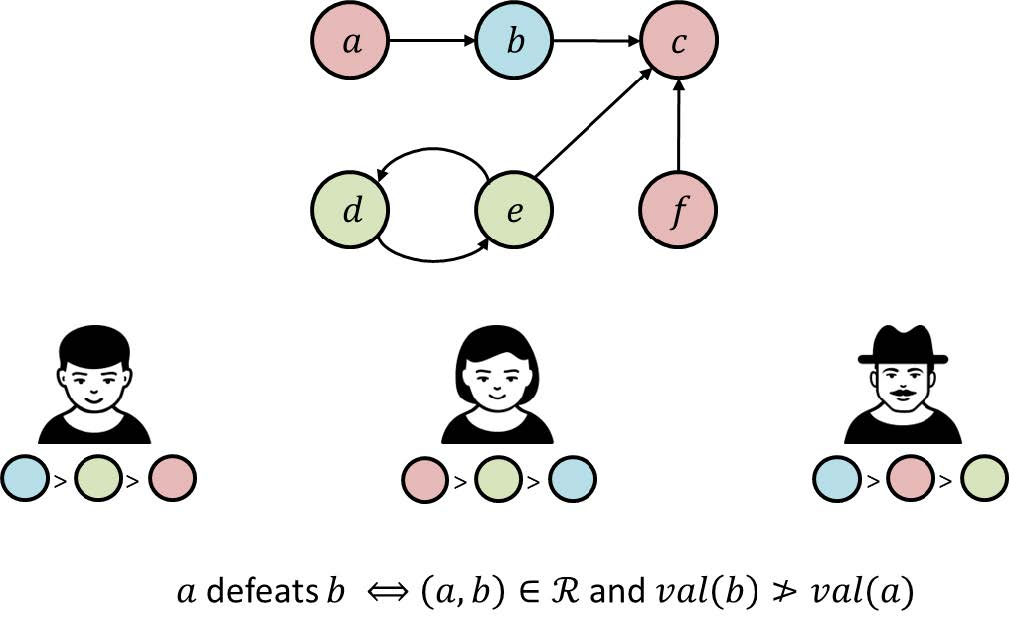
\includegraphics[width=0.5\textwidth]{Images/Value_based_AF.jpg}
    \caption{Value based argumentation framework}
\end{figure}

The Value-based Argumentation Framework (VAF) represents a crucial extension that introduces subjective evaluation into the reasoning process. Its strategic importance lies in its ability to model how different audiences, with different values or preferences, can arrive at different conclusions even when presented with the same set of arguments and attacks. This allows for a more realistic representation of debates where objectivity is not guaranteed. \\

A Value-Based Argumentation Framework (VAF) is a 5-tuple $VAF=⟨A,R,V,val,valpref⟩$. \\

Here, $⟨A,R⟩$ represents a standard argument framework, where $A$ is a set of arguments and $R$ is the attack relation between them. $V$ is a set of non-empty values (e.g., 'Liberty', 'Safety'), $val$ is a function that assigns a value from $V$ to each argument in $A$, and $valpref$ is a preference relation defining the hierarchy of those values for a specific audience. \\

The core mechanic of a VAF is its redefinition of a successful attack. In this model, an argument A only defeats argument B if A attacks B AND the value assigned to B is not preferred over the value assigned to A. In practical terms, this means that an attack originating from an argument with a "less important" value against an argument with a "more important" value can be disregarded, effectively removing that attack edge for that specific audience. \\

For example, consider an argumentation graph where arguments are mapped to values represented by colors (red, blue, yellow). Three different users, each with a unique preference ordering for these colors ($valpref$), will evaluate the same graph differently. \\

\begin{itemize}
    \item 
    \textbf{User 1 (\texttt{blue > yellow > red}):} An attack from a red argument to a blue argument fails because the target argument has a higher-preference value.

    \item 
    \textbf{User 2 (\texttt{red > yellow > blue}):} An attack from a yellow or blue argument to a red argument is ineffective.

    \item 
    \textbf{User 3 (\texttt{blue > red > yellow}):} An attack from a red or yellow argument to a blue one will fail to defeat it.
\end{itemize}

This illustrates how VAFs model subjectivity, showing that the same "objective" set of arguments and conflicts can lead to different sets of acceptable arguments depending on an individual's or group's value hierarchy. \\

While VAFs successfully add a layer of subjective preference, other frameworks were needed to model different types of relationships, such as explicit support between arguments.

\chapter{Modeling Agreement: The Bipolar Argumentation Framework (BAF)}

\begin{figure}[h]
    \centering
    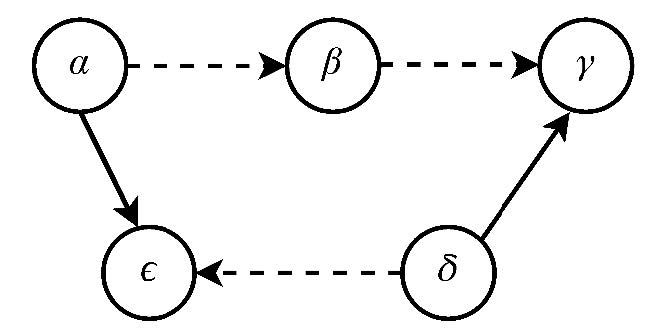
\includegraphics[width=0.5\textwidth]{Images/Bipolar_AF.jpg}
    \caption{Bipolar argumentation framework}
\end{figure}

The Bipolar Argumentation Framework (BAF) was developed to address a fundamental limitation of Dung's model: its inability to represent anything other than conflict. The key innovation of the BAF is the formal inclusion of an explicit support relation (represented with a dashed line), allowing the framework to capture both conflict (attack) and agreement (support) directly within the graph structure. \\

A Bipolar Argumentation Framework (BAF) is defined as $B=⟨A,R_{att},R_{sup}⟩$.\\

This structure consists of a set of arguments $A$, a binary attack relation $R_{att}$, and a binary support relation $R_{sup}$. \\

This dual-relation system enables the modeling of more complex interactions. For instance, two key patterns emerge:

\begin{itemize}
    \item 
    \textbf{Supported Attack:} An argument A supports an argument B, which in turn attacks argument C. In this scenario, A contributes to the attack on C.

    \item 
    \textbf{Indirect Attack:} An argument A attacks an argument B, which in turn supports argument C. Here, A indirectly weakens C by attacking one of its supporters.
\end{itemize}

\section{Advantages and Disadvantages of BAFs}

\begin{itemize}
    \item
    \textbf{Advantages:} The primary benefit of BAFs is their ability to model these more complex, combined interactions, providing a more expressive and realistic representation of debates where arguments can both attack and reinforce one another.

    \item 
    \textbf{Disadvantages:} Despite this added expressiveness, BAFs have notable limitations. There is a "hidden assumption" that conflict is inherently more powerful than support; a support relation can never cancel out or undo the effect of a direct attack. Furthermore, when using traditional extension-based semantics, all justified arguments are still treated as equally acceptable, providing no way to rank them or account for gradual levels of acceptability.
\end{itemize}

BAFs introduced the crucial concept of explicit support but lacked a mechanism to represent the varying strength of either attacks or supports, a gap addressed by Weighted Argumentation Frameworks.

\chapter{Quantifying Conflict: The Weighted Argumentation Framework (WAF)}

\begin{figure}[h]
    \centering
    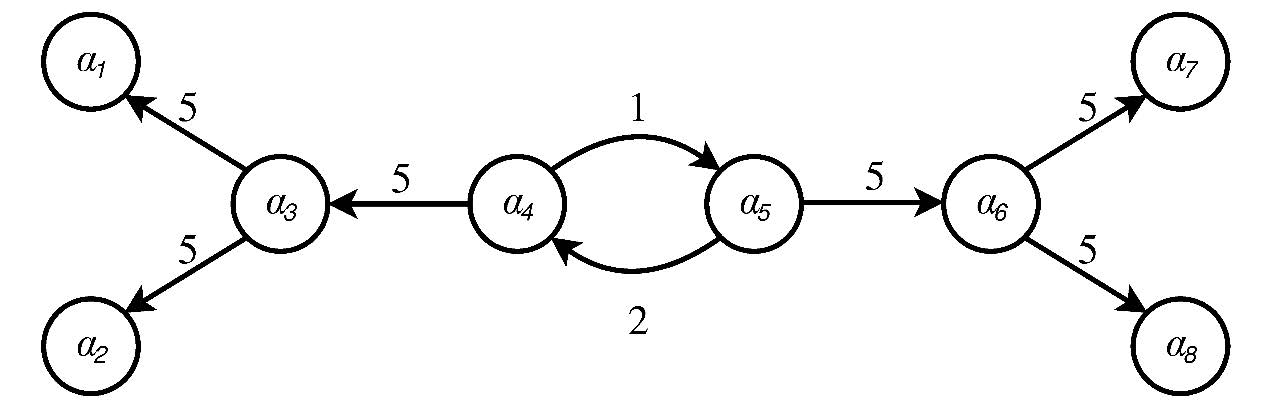
\includegraphics[width=0.5\textwidth]{Images/Weighted_AF.jpg}
    \caption{Weighted argumentation framework}
\end{figure}

The Weighted Argumentation Framework (WAF) enhances Dung's model by moving beyond a simple binary representation of conflict. This framework assigns a numerical weight to each attack, allowing it to represent its relative strength or importance. This enables a more granular analysis of the relationships between arguments. \\

A Weighted Argumentation Framework (WAF) is a triple $W=⟨A,R,w⟩$ where $⟨A,R⟩$ is a standard AF and $w:R \rightarrow R^+$ is a function assigning real-valued weights to attacks. \\

The primary mechanism for evaluating arguments in a WAF is the \textbf{Inconsistency Budget ($\beta$)}. This concept introduces the idea that a set of arguments can be considered collectively acceptable even if it contains some internal conflict, provided that the total conflict does not exceed a predefined threshold. The sum of the weights of all attacks between arguments within an extension must be less than or equal to the budget $\beta$.

\section{Advantages and Disadvantages of WAFs}

\begin{itemize}
    \item 
    \textbf{Advantages:} WAFs provide a method for selecting specific extensions by tolerating a certain degree of incoherence. This is particularly useful in scenarios where some level of internal conflict is realistic or unavoidable, allowing for a more flexible and pragmatic assessment of argument sets.

    \item
    \textbf{Disadvantages:} The model's design has significant drawbacks. First, it explicitly permits \textbf{non-conflict-free extensions}, which may be undesirable or logically inconsistent in many applications. Second, the weights assigned to attacks are not fully exploited; their only role is to be summed and checked against the inconsistency budget. They are not used, for example, to evaluate the cumulative strength of a path of attacks or to compare the impact of different lines of reasoning.
\end{itemize}

WAFs provide a solid foundation for quantifying the strength of conflict, but a more comprehensive model is needed to integrate both weighted attacks and weighted supports.

\chapter{The Integrated Model: The Bipolar Weighted Argumentation Framework (BWAF)}

\begin{figure}[h]
    \centering
    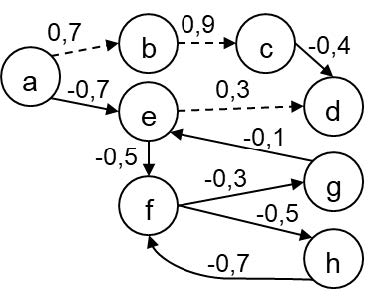
\includegraphics[width=0.5\textwidth]{Images/Bipolar_weighted_AF.jpg}
    \caption{Bipolar weighted argumentation framework}
\end{figure}

The Bipolar Weighted Argumentation Framework (BWAF) represents a powerful synthesis of the preceding models. Its strategic value lies in its ability to simultaneously model relationships of both weighted attack and weighted support, making it one of the most expressive frameworks for computational argumentation. It integrates the bipolar (attack/support) nature of BAFs with the quantitative strength representation of WAFs. \\

A Bipolar Weighted Argumentation Framework (BWAF) is a triple $G=\langle A,\hat{R},w_{\hat{R}} \rangle$ where $A$ is a finite set of arguments, $\hat{R} \subseteq A \times A$, and $w_{\hat{R}}:\hat{R} \rightarrow [-1,0) \cup (0,1]$ is a function assigning a weight to each relation. \\

A core convention of the BWAF is how it assigns weights. Negative weights in the range $[-1, 0)$ represent attacks of varying strengths (where the absolute value indicates strength), while positive weights in the range $(0, 1]$ represent supports of varying strengths. \\

One of the most significant advancements of the BWAF is its use of a path-based evaluation method. This approach determines the overall contribution of a sequence of arguments (a path) to a target argument's final acceptability. A simple and effective rule for this is to calculate the overall strength of a path by \textbf{multiplying the weights} of its constituent relations. If the final product is a negative value, the path represents an overall attack on the target argument. If the product is positive, the path contributes positively, acting as a defense or a complex support. This is the reason why the value $0$ is not included in the range of possible weights values. If an arc had a weight of $0$ it would nullify the overall weight of all the paths involving it.\\

This can be illustrated with an example targeting an argument D:

\begin{itemize}
    \item 
    A path \textbf{ABCD}, where A supports B, B supports C, and C attacks D (\texttt{$0.7 \cdot 0.9 \cdot -0.4$}), results in an overall strength of \textbf{$-0.252$}. This negative value indicates the path functions as a supported attack, reducing D's acceptability.

    \item 
    Another path \textbf{AED}, where A attacks E and E supports D (\texttt{$-0.7 \cdot 0.3$}), results in a strength of \textbf{$-0.21$}. This represents an indirect attack, also contributing negatively.

    \item
    A third path \textbf{FGED}, with weights \texttt{$-0.7, -0.1$}, and \texttt{$0.3$} along its edges, has a calculated strength of \texttt{$(-0.7) \cdot (-0.1) \cdot 0.3 = \textbf{+0.021}$}. The positive result signifies that this path, despite containing attacks, functions as a defense of D, contributing positively to its acceptability.
\end{itemize}

By summing the strength of all paths that terminate at a given argument, an overall acceptability score can be computed. When this process is applied to every argument in the framework, it yields a complete ranking of all arguments from most to least acceptable. \\

The BWAF thus represents a highly expressive and nuanced model, providing a sophisticated mechanism for analyzing complex argumentative scenarios.

\chapter{Comparative Summary of Argumentation Frameworks}

Table 16.1 provides a concise, at-a-glance comparison of the four advanced frameworks against the baseline limitations of Dung's original model.

\begin{table}[htbp]
    \centering
    \begin{tabularx}{\textwidth}{|X|X|X|X|} \hline
        \textbf{Framework} & \textbf{Core Problem Addressed} & \textbf{Key Mechanism} & \textbf{Primary Outcome} \\ \hline

        \textbf{Value-based AF (VAF)} &
        Lack of subjective preferences and audience-specific evaluation. &
        Assigns values to arguments and defines a preference order (\texttt{valpref}) over those values. &
        Audience-specific argument acceptance; an attack may fail if it comes from a less-preferred value. \\ \hline

        \textbf{Bipolar AF (BAF)} &
        No explicit representation of support relations. &
        Introduces a formal, explicit support relation ($R_{sup}$) alongside the attack relation. &
        Modeling of complex interactions like "supported attacks" and "indirect attacks." \\ \hline

        \textbf{Weighted AF (WAF)} &
        All attacks are treated as having equal strength. &
        Assigns a numerical weight to each attack and uses an "Inconsistency Budget" ($\beta$). &
        Acceptance of non-conflict-free argument sets, provided the total weight of internal attacks is below a threshold. \\ \hline

        \textbf{Bipolar Weighted AF (BWAF)} &
        Need to model both support/attack and their varying strengths simultaneously. &
        Assigns positive weights for support and negative weights for attack; calculates path strength via multiplication. &
        A comprehensive ranking of all arguments based on an aggregate score computed from all influencing paths. \\ \hline
    \end{tabularx}
    \caption{Argumentation frameworks comparison}
\end{table}

\end{document}
